\chapter{Compatibiliteit van herkenningssystemen}
Voor het herkenningssysteem bestuderen we de implementatie van de ResNet50 architectuur die in paragraaf \ref{resnet} werd besproken.
We vertrekken van een bestaand model dat voorgetraind is met het TensorFlow of het PyTorch framework om de verschillende mogelijkheden voor een mobiele implementatie te bestuderen.
Hierbij maken we gebruik van Google Colaboratory in CPU runtime om de modellen in te laden en te converteren.
Om het geconverteerd model te implementeren op een mobiel toestel maken we gebruik van Android Studio.
De ge\"implementeerde code is terug te vinden in de volgende github repository: \url{https://github.com/ThijsVercammen/Masterproef.git}.

% \section{ResNet50}
% \cite{he2015deep} heeft vastgesteld dat als het aantal lagen van een CNN toeneemt dat op een bepaald moment de training accuraatheid daalt.
% Dit verschijnsel noemt men de vanishing gradient.
% In paragraaf \ref{train} hebben we besproken hoe we de gradient kunnen berekenden tijdens het trainen van een CNN.
% Voor elke laag in het CNN moet de gradient opnieuw berekend worden door telkens opnieuw de afgeleide te berekenen.
% Hierdoor wordt de gradient steeds kleiner en kleiner tot deze een minimum bereikt.
% Waardoor de gewichten in de eerste lagen heel traag aanpassen of zelfs niet meer veranderen.
% \cite{he2015deep} die dit probleem hebben vastgesteld hebben dit opgelost door gebruik te maken van skip connections.
% Hierbij wordt de input van een laag rechtstreeks met een volgende laag die x aantal lagen verder ligt.
% Op deze manier worden de gradienten per laag niet meer kleiner.
% ResNet50 bestaat uit 50 convolutie lagen waarbij er een skip connection plaatsvindt per 3 lagen.
% De resnet50 architectuur is opgebouwd uit ResNet blokken die bestaan uit 3 convolutie lagen en 1 skip connection.

%https://github.com/tensorflow/models/blob/master/official/vision/image_classification/resnet/resnet_model.py
%https://github.com/priya-dwivedi/Deep-Learning/blob/master/resnet_keras/Residual_Networks_yourself.ipynb

\section{Van TensorFlow naar mobiel framework}
Voor het experiment van ResNet50 maken gebruiken we het standaard ResNet50 netwerk dat in TensorFlow ge\"implementeerd kan worden vanuit Keras.
Dit ResNet50 model is voorgetrained op de ImageNet dataset \cite{deng_2009_imagenet}. 
Dit netwerk kunnen we vervolgens hertrainen naar een gewenste functionaliteit.
Voor deze implementatie zullen we echter vertrekken van het ResNet50 Keras model dat reeds bestaat.

\subsection{TensorFlow Lite implementatie} \label{tf_h_conv}
Het inladen en converteren van het Keras model kan eenvoudig via de volgende Python code.

\begin{python}
model = tf.keras.applications.resnet50.ResNet50() # model inladen
converter = tf.lite.TFLiteConverter.from_keras_model(model) # init converter
tflite_model = converter.convert() # model converteren
open('model.tflite', 'wb').write(tflite_model) # model opslaan
\end{python}

Het ResNet50 model kan zonder problemen of aanpassingen rechtstreeks worden geconverteerd naar TFlite.
We vertrekken van een bestaand model dat voorgetraind is met het TensorFlow of het PyTorch framework om de verschillende mogelijkheden voor een mobiele implementatie te bestuderen.
In de tabel kunnen we zien welke TensorFlow operaties worden ondersteund door een TFLite equivalent.
Verder is in de tabel weergegeven welke TensorFlow operaties worden ondersteund door een TFLite equivalent en op welke operaties optimalisaties worden uitgevoerd tijdens het converteren. 
Bij deze optimalisaties worden operaties samengevoegd, verwijderd of vervangen door een constante.
Figuur \ref{fig:class_opt} laat zien welke optimalisaties er worden uitgevoerd op een ResNet50 convolutieblok.

\begin{figure}[!ht]
	\centering
	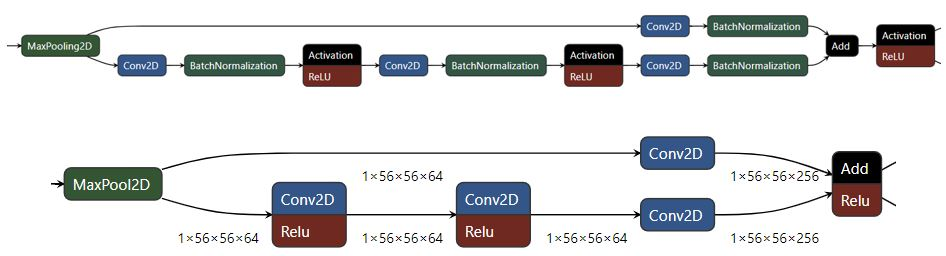
\includegraphics[width=1.0\linewidth]{fig/class_opt.jpg}
	\caption{ResNet50 convolutieblok voor en na TFLite conversie. BatchNorm en ReLu zijn hierbij samengevoegd met de Conv2D opperaties.}
	\label{fig:class_opt}
\end{figure}

Voor de android implementatie kunnen we metadata aan het model toevoegen.
Dit is niet noodzakelijk, maar vereenvoudigd de Android implementatie.
\begin{python} 
ImageClassifierWriter = image_classifier.MetadataWriter
model_p = "./model.tflite" # TFLite model
label_p = "./labels.txt" # label file voor label formaat
save_p = "./model_meta.tflite" # opslaan pad
input_norm_mean = 0.0
input_norm_std = 1.0
    
# metadata scrijver
writer = ImageClassifierWriter.create_for_inference(
    writer_utils.load_file(model_p), [input_norm_mean], [input_norm_std],
    [label_p])
    
# Voeg metadata aan het model toe en sla op
writer_utils.save_file(writer.populate(), save_p)
\end{python}

Omdat we deze metadata hebben toegevoegd heeft Android studio toegang tot al de relevante input en output informatie.
Vermits Android studio toegang heeft tot deze informatie kan het zelf code genereren om het TFLite model te implementeren.
De code die gegenereerd wordt is implementeerbaar in Java en Kotlin.
Onderstaande Java code heeft Android studio voor ons gegenereerd.
Het enige wat nu nog rest is een afbeelding inlezen als bitmap en de output afhandelen.
\begin{python}
Model model = Model.newInstance(context);

// Creates inputs for reference.
TensorImage image = TensorImage.fromBitmap(bitmap);

// Runs model inference and gets result.
Model.Outputs outputs = model.process(image);
List<Category> probability = outputs.getProbabilityAsCategoryList();

// Releases model resources if no longer used.
model.close();
\end{python}

\begin{table}[!ht]
    \caption{Alle operaties die terug te vinden zijn in het TensorFlow ResNet50 model en hun compatibiliteit met andere frameworks}
\begin{tabular}{ccc}
    \hline
    TensorFlow Operaties & TensorFlow \textrightarrow TFLite & ONNX Opset \\
    \hline
    AddV2 & Ondersteund & 1 \\
    BiasAdd & Samengevoegd & 1 \\
    %Const & constant & 1 \\
    Conv2D & Ondersteund & 1 \\
    FusedBatchNormV3 & Samengevoegd & 6 \\
    Identity & Verwijderd & 1 \\
    MatMul & Ondersteund & 1 \\
    MaxPool & Ondersteund & 1 \\
    Mean & Ondersteund & 1 \\
    NoOp & Verwijderd & / \\
    %Pack & Ondersteund & 1 \\
    Pad & Ondersteund & 1 \\
    Placeholder & Constant & 1 \\
    Relu & Samengevoegd & 1 \\
    Softmax & Ondersteund & 1 \\
    %StatefulPartitionedCall & Ondersteund & / \\
    \hline
\end{tabular}
\label{tab:TFop}
\end{table}

\subsection{ONNX implementatie} \label{classonnx}
Het TensorFlow model kunnen we converteren naar ONNX met tf2onnx bibliotheek.
De tf2onnx bibliotheek ondersteunt TensorFlow en TFLite.
Hierdoor kunnen we beide modellen converteren naar ONNX.
In tabel \ref{tab:TFop} kunnen we afleiden welke operaties ondersteund zijn door ONNX en vanaf welke opset versie deze operaties worden ondersteund.
De minimale opset moet versie 6 zijn vanwege de FusedBatchNormV3 operatie die pas vanaf versie 6 wordt ondersteund.
Via het volgende CLI commando kunnen we het TensorFlow model converteren naar ONNX of kunnen we het TFLite model converteren naar ONNX door de optie --tflite mee te geven.

\begin{python}
python -m tf2onnx.convert --saved-model ./model --output model.onnx
\end{python}

Voor de Android implementatie van het ONNX model maken we gebruik van Kotlin in plaats van Java.
De voornaamste reden hiervoor is dat de Onnxruntime documentatie Kotlin code gebruikt voor de Java API.
%voorbeelden ook in Kotlin zijn ge\"implementeerd.
Via onderstaande Kotlin code kan het ONNX model worden uitgevoerd in Android studio.

\begin{python} 
var env = OrtEnvironment.getEnvironment()
// lees het ONNX model als byteArray
var session = env.createSession(resources.openRawResource(R.raw.model_tf).readBytes())
// Maak een input tensor aan
var input_tensor = OnnxTensor.createTensor(env, imgData, shape)
// maak een inputmap aan
var inputs = Collections.singletonMap("input_1", t1)
// voer model uit
val output = session?.run(inputs)
\end{python}

We lezen het ONNX model in als een byteArray.
Dit ONNX model hebben we opgeslagen in de res/raw folder van het Android studio project.
Vervolgens wordt er een ONNX input tensor aangemaakt.
Hierbij wordt de data van de afbeelding als FloatArray meegegeven net als de vorm van de input tensor die het ONNX model verwacht.
Het ONNX model verwacht een input vorm [1, hoogte, breedte, 3] deze vorm is van het NHWC formaat eerder besproken in \ref{nhwc}.
Voordat we het model kunnen uitvoeren moeten we de input tensor aan een map toevoegen.
De keys van deze map zijn de namen van de inputs die het ONNX model verwacht, de values van de map zijn de input tensoren.
De input namen zijn terug te vinden in de output boodschappen van tf2onnx converter.
%We moeten er wel bij vermelden dat TFLite enkel variabelen van het type float32 en int8 ondersteund.
%De tf2onnx converter maakt standaard gebruik van ONNX opset versie 9.
%Bij het converterent van TensorFlow naar ONNX onder standaard omstandigheden krijgen we de volgende fout 
%\textcolor{red}{ValueError: StridedSlice: only strides=1 is supported}.  
%Voor het converteren van TensorFlow naar ONNX is minstens opset versie 10 nodig.

\section{Van PyTorch naar mobiele implementatie}
Voor de PyTorch implementatie gebruiken we van het ResNet50 model uit de Torchvision bibliotheek.
Dit model is voorgetraind op de ImageNet dataset (\cite{deng_2009_imagenet}) .
Dit netwerk kunnen we vervolgens hertrainen voor een gewenste functionaliteit.
Voor deze implementatie zullen we echter vertrekken van het reeds bestaande ResNet50 Torchvision model.

\subsection{PyTorch Mobile implementatie} \label{py_class}
Via de volgende Python code kunnen we een ResNet50 Torchvision model inladen en converteren voor mobiel gebruik.

\begin{python}
model = models.resnet50(pretrained=True) # model inladen
model.eval() # model in uitvoer modus
example = torch.rand(1, 3, 224, 224) # voorbeeld input
# Torchscript module genereren
traced_script_module = torch.jit.trace(model, example) 
# optimalisaties voor mobiel gebruik uitvoeren op de scriptmodule
traced_script_module_optimized = optimize_for_mobile(traced_script_module)
# model opslaan voor mobiel gebruik
traced_script_module_optimized._save_for_lite_interpreter("./model.pt") 
\end{python}

Het ResNet50 model wordt zonder problemen geconverteerd, geoptimaliseerd en opgeslagen voor mobiel gebruik.
In tabel \ref{tab:PYop} zien we welke operaties er terug te vinden zijn in het Torchvision model en wat er met deze operaties gebeurt tijdens de conversie.
Het mobiel model kunnen we vervolgens implementeren in Android studio.

\begin{table}[!ht]
    \caption{Alle operaties die terug te vinden zijn in het Torchvision ResNet50 model en hun compatibiliteit met andere frameworks}
\begin{tabular}{ccc}
    \hline
    TorchScript & TorchScript \textrightarrow  ge\"optimaliseerd torchscript & ONNX Opset \\
    \hline
    Add & Ondersteund & 1 \\
    AdaptiveAvgPool2d & Ondersteund & 1 \\
    BatchNorm2d & Samengevoegd & 1 \\
    Conv2d & Ondersteund & 1 \\
    Flatten & Ondersteund & 1 \\
    Linear & Ondersteund & 1 \\
    MaxPool2d & Ondersteund & 1 \\
    ReLu & Samengevoegd & 1 \\
    \hline
\end{tabular}
\label{tab:PYop}
\end{table}

Het ResNet50 Torchvision model verwacht een genormaliseerde input dat standaard is voor elk Torchvision model.
Door de input te normaliseren verwacht het model altijd een pixelwaarde met een gemiddelde van 0 en een standaarddeviatie van 1.

\begin{equation}
    \begin{aligned}
	\textrm{TORCHVISION\_NORM\_MEAN\_RGB}  = \{0.485, 0.456, 0.406\} \\
	\textrm{TORCHVISION\_NORM\_STD\_RGB}  = \{0.229, 0.224, 0.225\}
    \end{aligned}
\end{equation}

Het model kan vervolgens met de volgende Java code eenvoudig ge\"implementeerd worden in Android studio. 

\begin{python}
module = Module.load(assetFilePath(MainActivity.this, "model.ptl"));
Tensor inputTensor = TensorImageUtils.bitmapToFloat32Tensor(bitmap,
            TensorImageUtils.TORCHVISION_NORM_MEAN_RGB, 
            TensorImageUtils.TORCHVISION_NORM_STD_RGB);
Tensor outputTensor = module.forward(IValue.from(inputTensor)).toTensor();
\end{python}

\subsection{ONNX implementatie} \label{py_onnx}
Het ResNet50 Torchvision model kunnen we in Python eenvoudig converteren naar ONNX via de volgende code:

\begin{python}
torch.onnx.export(model, # model 
    example,             # model input
    "model_py.onnx",     # waar opslaan
    input_names = ['input_1'], # input namen
    output_names = ['output']) # output namen    
\end{python}

Het gegenereerde ONNX model kan ge\"implementeerd worden in Android studio.
Het ONNX model verwacht een input vorm [1, 3, hoogte, breedte], deze vorm is van het NCHW formaat eerder besproken in \ref{nhwc}.
Het geconverteerd PyTorch model verwacht een genormaliseerde input van een afbeelding.
De genormaliseerde waarde kan via de volgende formule berekend worden.

\begin{equation}
    \begin{aligned}
	\textrm{genormaliseerd}  = \frac{(\textrm{waarde} - \textrm{mean})}{\textrm{std}} \\
    \textrm{mean}  = \{0.485, 0.456, 0.406\} \\
	\textrm{std}  = \{0.229, 0.224, 0.225\}
\end{aligned}
\end{equation}

In deze formule is mean de gemiddelde waarde en std de standaarddeviatie waarmee Torchvision een normalisatie uitvoert.
De mean en std bevatten drie waarde.
Dit is omdat bij Torchvision elk kleurkanaal zijn eigen mean en std waarde heeft voor normalisatie.
De rest van de implementatie in Android studio is identiek aan de ONNX implementatie van het TensorFlow model zoals besproken in \ref{classonnx}. 

\section{Samenvatting}
We hebben gezien dat herkenningssystemen volledig ondersteund zijn.
De modellen van het PyTorch en TensorFlow framework worden zonder problemen geconverteerd naar een model voor mobiel gebruik.

Voor het TensorFlow model kunnen we in Python ons model converteren met de onderstaande code.
Dit model is implementeerbaar in Android studio.
TensorFlow geeft ons de mogelijkheid om hier Metadata aan toe te voegen, waardoor Android studio de nodige code voor ons genereert.

\begin{python}
    converter = tf.lite.TFLiteConverter.from_keras_model(model)
    tflite_model = converter.convert()
    open('model.tflite', 'wb').write(tflite_model) # model opslaan
\end{python}

Het PyTorch model kunnen we ook eenvoudig converteren met onderstaande Python code.
We moeten wel rekening houden met het feit dat het Torchvision model een genormaliseerde input verwacht.

\begin{python}
model.eval() # model in uitvoer modus
example = torch.rand(1, 3, 224, 224) # voorbeeld input
traced_script_module = torch.jit.trace(model, example) 
traced_script_module_optimized = optimize_for_mobile(traced_script_module)
traced_script_module_optimized._save_for_lite_interpreter("./model.pt") 
\end{python}

Het TensorFlow model kan naar ONNX geconverteerd worden via het volgende CLI-commando.

\begin{python}
python -m tf2onnx.convert --saved-model ./model --output model.onnx
\end{python}

Voor PyTorch gebeurt de conversie naar ONNX via onderstaande Python code.

\begin{python}
torch.onnx.export(model, example, "model.onnx",
        input_names = ['input'], output_names = ['output'])    
\end{python}

De twee ONNX modellen worden op dezelfde ge\"implementeerd in Android studio.
Hierbij moeten we wel rekening houden met het input formaat.
Het PyTorch ONNX model verwacht NCHW formaat en het TensorFlow ONNX model verwacht NHWC formaat.
Bovendien verwacht het PyTorch ONNX model een genormaliseerde input en het TensorFlow ONNX model geen genormaliseerde input.